\section{Event Yields and Background Estimation}
\label{sec:yields}

In the following Tables~\ref{tab:yield_baseline} 
to~\ref{tab:yield_ht200met503btag}
we summarize the background 
estimates and compare them to the
observed counts of events in data for the baseline and search region selections
defined in Sections~\ref{sec:eventsel} and~\ref{sec:regions}.
In each table the expectations from the simulation alone are given 
in the upper part.
 These are used to get a feeling of the expected contributions.
Among these MC expectations, 
only those with actual final state 
isolated same-sign leptons are used for the final result
as described in Section~\ref{sec:bkgds}.
The lower part of each table is the main result of the analysis
used for comparisons with data and setting constraints on various models.
These include the predictions for the fake-lepton and charge misidentification
bacgrounds derived as described in Section~\ref{sec:datadriven}.

To reiterate and make it absolutely clear.  The total background
prediction in a given signal region
is the sum of three distinct components:
\begin{enumerate}

\item The data-driven charge misid prediction (row ``Charge Flips'' in
Tables~\ref{tab:yield_baseline} to~\ref{tab:yield_ht320met120}).

\item The data-driven sum of single fakes (SF) and double fakes
(DF) predictions (row ``SF$+$DF''
in Tables~\ref{tab:yield_baseline} to~\ref{tab:yield_ht320met120}).

\item The total MC prediction for processes that naturally give isolated
same sign dileptons, see Section~\ref{sec:bkgds} (row ``MC Pred'' in
Tables~\ref{tab:yield_baseline} to~\ref{tab:yield_ht320met120};
this is the sum of the rows starting from ``$V\gamma$'' down to 
and including the tribosons -- although in practice only $ttW$ and 
$ttZ$ matter).  Note that for the dominant physics 
backgrounds we normalized the MC to $\sigma(pp \to ttW) = 0.1633 \pm 0.082$
pb and $\sigma(pp \to ttZ) = 0.139 \pm 0.070$ pb.

\end{enumerate}

Details on the systematics of the background predictions are given in the corresponding sections.
The final estimates on these uncertainties are rather simple:
\begin{enumerate}
\item The charge flip contribution has a 20\% systematics.
  \item The predicted number of fakes has a 50\% systematics in all modes.
  \item The MC prediction for ``real'' same sign isolated dileptons
    has an uncertainty of 50\%.
  
\end{enumerate}

\newcommand{\ttdilS}{\ensuremath{\ttbar\to\ell\ell X}}
\newcommand{\ttslbS}{\ensuremath{\ttbar\to\ell(b\to\ell) X}}
\newcommand{\ttsloS}{\ensuremath{\ttbar\to\ell(b\!\!\!/\to\ell) X}}
\newcommand{\SFnn}{\ensuremath{N^{\rm Wj,raw}_{nn}}}

\begin{table}[h]
\begin{center}
\begin{tabular}{l | l l l l}
\hline\hline
 Source  &  ee  &  $\mu\mu$  &  e$\mu$  &  all \\
\hline
$t\overline{t}\rightarrow \ell\ell X$ &  0.469 $\pm$  0.305 &  0.000 $\pm$  0.199 &  1.133 $\pm$  0.580 &  1.603 $\pm$  0.656\\
$t\overline{t}$ other &  0.000 $\pm$  0.199 &  0.000 $\pm$  0.199 &  0.000 $\pm$  0.199 &  0.000 $\pm$  0.199\\
$t\overline{t}\rightarrow \ell(b\rightarrow \ell)X$ &  0.000 $\pm$  0.199 &  0.193 $\pm$  0.143 &  0.000 $\pm$  0.199 &  0.193 $\pm$  0.143\\
$t\overline{t}\rightarrow \ell(\slashed{b}\rightarrow \ell)X$ &  0.563 $\pm$  0.399 &  0.000 $\pm$  0.199 &  0.143 $\pm$  0.131 &  0.706 $\pm$  0.420\\
\hline
$t$, s-channel &  0.000 $\pm$  0.057 &  0.000 $\pm$  0.057 &  0.000 $\pm$  0.057 &  0.000 $\pm$  0.057\\
$t$, t-channel &  0.077 $\pm$  0.077 &  0.000 $\pm$  0.055 &  0.000 $\pm$  0.055 &  0.077 $\pm$  0.077\\
$tW$ &  0.000 $\pm$  0.045 &  0.000 $\pm$  0.045 &  0.016 $\pm$  0.045 &  0.016 $\pm$  0.045\\
\hline
$Z\rightarrow ee$ &  0.000 $\pm$  0.429 &  0.000 $\pm$  0.429 &  0.000 $\pm$  0.429 &  0.000 $\pm$  0.429\\
$Z\rightarrow\mu\mu$ &  0.000 $\pm$  0.429 &  0.000 $\pm$  0.429 &  0.000 $\pm$  0.429 &  0.000 $\pm$  0.429\\
$Z\rightarrow\tau\tau$ &  0.000 $\pm$  0.429 &  0.000 $\pm$  0.429 &  0.000 $\pm$  0.429 &  0.000 $\pm$  0.429\\
$W$+jets &  0.000 $\pm$  1.808 &  0.000 $\pm$  1.808 &  0.000 $\pm$  1.808 &  0.000 $\pm$  1.808\\
$WW$ &  0.000 $\pm$  0.019 &  0.000 $\pm$  0.019 &  0.000 $\pm$  0.019 &  0.000 $\pm$  0.019\\
\hline
V$\gamma$ &  0.000 $\pm$  0.248 &  0.000 $\pm$  0.248 &  0.000 $\pm$  0.248 &  0.000 $\pm$  0.248\\
$W\gamma^{*}\rightarrow\ell\nu e e$ &  0.000 $\pm$  0.097 &  0.000 $\pm$  0.097 &  0.000 $\pm$  0.097 &  0.000 $\pm$  0.097\\
$W\gamma^{*}\rightarrow\ell\nu\mu\mu$ &  0.000 $\pm$  0.075 &  0.000 $\pm$  0.075 &  0.000 $\pm$  0.075 &  0.000 $\pm$  0.075\\
$W\gamma^{*}\rightarrow\ell\nu\tau\tau$ &  0.000 $\pm$  0.028 &  0.000 $\pm$  0.028 &  0.000 $\pm$  0.028 &  0.000 $\pm$  0.028\\
$WZ$ &  0.034 $\pm$  0.012 &  0.017 $\pm$  0.008 &  0.031 $\pm$  0.012 &  0.082 $\pm$  0.019\\
$ZZ$ &   0.000 $\pm$   0.000 &  0.001 $\pm$  0.001 &  0.002 $\pm$  0.001 &  0.003 $\pm$  0.001\\
\hline
dp$W^{\pm}W^{\pm}$ &  0.000 $\pm$  0.004 &  0.000 $\pm$  0.004 &  0.000 $\pm$  0.004 &  0.000 $\pm$  0.004\\
sp$W^{-}W^{-}$ &  0.000 $\pm$  0.001 &  0.000 $\pm$  0.001 &  0.003 $\pm$  0.002 &  0.003 $\pm$  0.002\\
sp$W^{+}W^{+}$ &  0.000 $\pm$  0.006 &  0.000 $\pm$  0.006 &  0.000 $\pm$  0.006 &  0.000 $\pm$  0.006\\
$t\overline{t}\gamma$ &  0.000 $\pm$  0.059 &  0.000 $\pm$  0.059 &  0.000 $\pm$  0.059 &  0.000 $\pm$  0.059\\
$t\overline{t}W$ &  0.572 $\pm$  0.025 &  0.733 $\pm$  0.028 &  1.286 $\pm$  0.038 &  2.591 $\pm$  0.053\\
$t\overline{t}Z$ &  0.118 $\pm$  0.009 &  0.158 $\pm$  0.010 &  0.268 $\pm$  0.013 &  0.544 $\pm$  0.019\\
$WW\gamma$ &  0.000 $\pm$  0.015 &  0.000 $\pm$  0.015 &  0.000 $\pm$  0.015 &  0.000 $\pm$  0.015\\
$WWW$ &  0.001 $\pm$   0.000 &  0.001 $\pm$   0.000 &  0.001 $\pm$  0.001 &  0.003 $\pm$  0.001\\
$WWZ$ &   0.000 $\pm$   0.000 &   0.000 $\pm$   0.000 &  0.001 $\pm$  0.001 &  0.001 $\pm$  0.001\\
$WZZ$ &   0.000 $\pm$   0.000 &  0.001 $\pm$   0.000 &  0.001 $\pm$   0.000 &  0.002 $\pm$  0.001\\
$ZZZ$ &   0.000 $\pm$   0.000 &   0.000 $\pm$   0.000 &   0.000 $\pm$   0.000 &   0.000 $\pm$   0.000\\
\hline
Total MC &  1.834 $\pm$  0.509 &  1.103 $\pm$  0.146 &  2.885 $\pm$  0.597 &  5.822 $\pm$  0.797\\
\hline\hline
\hline
LM6 &  0.000 $\pm$  0.000 &  0.186 $\pm$  0.186 &  0.383 $\pm$  0.275 &  0.569 $\pm$  0.332\\
\hline\hline
\hline\hline
 SF  & 1.13 $\pm$ 0.67 & 0.30 $\pm$ 0.20 & 1.92 $\pm$ 0.74 & 3.36 $\pm$ 1.02\\
 DF  & 0.04 $\pm$ 0.12 & 0.02 $\pm$ 0.02 & 0.02 $\pm$ 0.09 & 0.08 $\pm$ 0.16\\
\hline
 SF + DF  & 1.17 $\pm$ 0.63 $\pm$ 0.58 & 0.32 $\pm$ 0.20 $\pm$ 0.16 & 1.95 $\pm$ 0.72 $\pm$ 0.97 & 3.43 $\pm$ 0.98 $\pm$ 1.72\\
\hline\hline
Charge Flips & 0.390 $\pm$ 0.032 $\pm$ 0.078 & - $\pm$ - & 0.544 $\pm$ 0.032 $\pm$ 0.109 & 0.934 $\pm$ 0.045 $\pm$ 0.187\\
\hline\hline
\hline
MC Pred &  0.725 $\pm$  0.029 $\pm$  0.362 &  0.912 $\pm$  0.031 $\pm$  0.456 &  1.595 $\pm$  0.042 $\pm$  0.797 &  3.231 $\pm$  0.059 $\pm$  1.616\\
\hline\hline
Total Pred &  2.281 $\pm$  0.633 $\pm$  0.691 &  1.232 $\pm$  0.199 $\pm$  0.483 &  4.086 $\pm$  0.725 $\pm$  1.263 &  7.600 $\pm$  0.983 $\pm$  2.365\\
\hline\hline
data & 2 & 2 & 3 & 7\\
\hline\hline
\end{tabular}

\end{center}
\caption{\label{tab:yield_baseline}Observed event yields in baseline 
(\met $>$ 30 GeV, at least 2 jets with pT $>$ 40 GeV, and at least two of these jets b-tagged using SSVHEM) 
high-\pt\ (pT $>$ 20/20) dileptons
compared to expectations from simulation alone, and from the data-driven methods.
The upper part of the table is based on simulation only and is used only as a reference.
The lower part is the main result of the analysis.
The SF (DF) contributions are for events with one (two) fake leptons.
The {\em MC Pred} contribution includes contributions from genuine  same-sign lepton
pairs (a sum of the rows from $V\gamma$ down to $ZZZ$).
Entries with zero contributing events are reported with an uncertainty corresponding to one event.
This uncertainty is not added to the total MC contribution.
Systematic uncertainties (the second uncertainty if present)
 are displayed only for the final combined type of background, no systematic
uncertainty is added for estimates with zero entries.
Systematic uncertainties are 100\% correlated among the channels.
}
\end{table}

\clearpage

\begin{table}[h]
\begin{center}
\begin{tabular}{l | l l l l}
\hline\hline
 Source  &  ee  &  $\mu\mu$  &  e$\mu$  &  all \\
\hline
$t\overline{t}\rightarrow \ell\ell X$ &  0.406 $\pm$  0.089 &  0.000 $\pm$  0.014 &  0.442 $\pm$  0.091 &  0.848 $\pm$  0.127\\
$t\overline{t}$ other &  0.000 $\pm$  0.014 &  0.000 $\pm$  0.014 &  0.000 $\pm$  0.014 &  0.000 $\pm$  0.014\\
$t\overline{t}\rightarrow \ell(b\rightarrow \ell)X$ &  0.040 $\pm$  0.029 &  0.101 $\pm$  0.044 &  0.027 $\pm$  0.027 &  0.168 $\pm$  0.059\\
$t\overline{t}\rightarrow \ell(\slashed{b}\rightarrow \ell)X$ &  0.367 $\pm$  0.083 &  0.005 $\pm$  0.014 &  0.343 $\pm$  0.080 &  0.715 $\pm$  0.115\\
\hline
$t$, s-channel &  0.000 $\pm$  0.061 &  0.000 $\pm$  0.061 &  0.000 $\pm$  0.061 &  0.000 $\pm$  0.061\\
$t$, t-channel &  0.000 $\pm$  0.058 &  0.000 $\pm$  0.058 &  0.000 $\pm$  0.058 &  0.000 $\pm$  0.058\\
$tW$ &  0.000 $\pm$  0.049 &  0.000 $\pm$  0.049 &  0.000 $\pm$  0.049 &  0.000 $\pm$  0.049\\
\hline
$Z\rightarrow ee$ &  0.000 $\pm$  0.458 &  0.000 $\pm$  0.458 &  0.000 $\pm$  0.458 &  0.000 $\pm$  0.458\\
$Z\rightarrow\mu\mu$ &  0.000 $\pm$  0.458 &  0.000 $\pm$  0.458 &  0.000 $\pm$  0.458 &  0.000 $\pm$  0.458\\
$Z\rightarrow\tau\tau$ &  0.000 $\pm$  0.458 &  0.000 $\pm$  0.458 &  0.000 $\pm$  0.458 &  0.000 $\pm$  0.458\\
$W$+jets &  0.000 $\pm$  1.932 &  0.000 $\pm$  1.932 &  0.000 $\pm$  1.932 &  0.000 $\pm$  1.932\\
$WW$ &  0.000 $\pm$  0.020 &  0.000 $\pm$  0.020 &  0.000 $\pm$  0.020 &  0.000 $\pm$  0.020\\
\hline
V$\gamma$ &  0.000 $\pm$  0.265 &  0.000 $\pm$  0.265 &  0.000 $\pm$  0.265 &  0.000 $\pm$  0.265\\
$W\gamma^{*}\rightarrow\ell\nu e e$ &  0.000 $\pm$  0.104 &  0.000 $\pm$  0.104 &  0.000 $\pm$  0.104 &  0.000 $\pm$  0.104\\
$W\gamma^{*}\rightarrow\ell\nu\mu\mu$ &  0.000 $\pm$  0.080 &  0.000 $\pm$  0.080 &  0.000 $\pm$  0.080 &  0.000 $\pm$  0.080\\
$W\gamma^{*}\rightarrow\ell\nu\tau\tau$ &  0.000 $\pm$  0.030 &  0.000 $\pm$  0.030 &  0.000 $\pm$  0.030 &  0.000 $\pm$  0.030\\
$WZ$ &  0.012 $\pm$  0.007 &  0.005 $\pm$  0.004 &  0.016 $\pm$  0.008 &  0.033 $\pm$  0.011\\
$ZZ$ &   0.000 $\pm$   0.000 &   0.000 $\pm$   0.000 &  0.001 $\pm$  0.001 &  0.001 $\pm$  0.001\\
\hline
dp$W^{\pm}W^{\pm}$ &  0.000 $\pm$  0.005 &  0.000 $\pm$  0.005 &  0.000 $\pm$  0.005 &  0.000 $\pm$  0.005\\
sp$W^{-}W^{-}$ &  0.000 $\pm$  0.002 &  0.000 $\pm$  0.002 &  0.000 $\pm$  0.002 &  0.000 $\pm$  0.002\\
sp$W^{+}W^{+}$ &  0.000 $\pm$  0.006 &  0.000 $\pm$  0.006 &  0.000 $\pm$  0.006 &  0.000 $\pm$  0.006\\
$t\overline{t}\gamma$ &  0.000 $\pm$  0.063 &  0.000 $\pm$  0.063 &  0.000 $\pm$  0.063 &  0.000 $\pm$  0.063\\
$t\overline{t}W$ &  0.451 $\pm$  0.023 &  0.537 $\pm$  0.024 &  0.960 $\pm$  0.033 &  1.947 $\pm$  0.047\\
$t\overline{t}Z$ &  0.062 $\pm$  0.007 &  0.080 $\pm$  0.008 &  0.143 $\pm$  0.010 &  0.285 $\pm$  0.014\\
$WW\gamma$ &  0.000 $\pm$  0.016 &  0.000 $\pm$  0.016 &  0.000 $\pm$  0.016 &  0.000 $\pm$  0.016\\
$WWW$ &  0.001 $\pm$   0.000 &  0.001 $\pm$   0.000 &  0.001 $\pm$  0.001 &  0.002 $\pm$  0.001\\
$WWZ$ &   0.000 $\pm$   0.000 &   0.000 $\pm$   0.000 &  0.000 $\pm$   0.000 &   0.000 $\pm$   0.000\\
$WZZ$ &   0.000 $\pm$   0.000 &  0.001 $\pm$   0.000 &   0.000 $\pm$   0.000 &  0.002 $\pm$  0.001\\
$ZZZ$ &   0.000 $\pm$   0.000 &   0.000 $\pm$   0.000 &   0.000 $\pm$   0.000 &   0.000 $\pm$   0.000\\
\hline
Total MC &  1.339 $\pm$  0.127 &  0.730 $\pm$  0.051 &  1.933 $\pm$  0.129 &  4.002 $\pm$  0.188\\
\hline\hline
\hline
LM6 &  0.000 $\pm$  0.000 &  0.199 $\pm$  0.199 &  0.240 $\pm$  0.240 &  0.438 $\pm$  0.311\\
\hline\hline
\hline\hline
 SF  & 0.06 $\pm$ 0.50 & 0.30 $\pm$ 0.20 & 1.32 $\pm$ 0.66 & 1.69 $\pm$ 0.85\\
 DF  & 0.04 $\pm$ 0.12 & 0.02 $\pm$ 0.02 & 0.02 $\pm$ 0.09 & 0.08 $\pm$ 0.16\\
\hline
 SF + DF  & 0.10 $\pm$ 0.45 $\pm$ 0.05 & 0.32 $\pm$ 0.20 $\pm$ 0.16 & 1.34 $\pm$ 0.64 $\pm$ 0.67 & 1.76 $\pm$ 0.80 $\pm$ 0.88\\
\hline\hline
Charge Flips & 0.255 $\pm$ 0.018 $\pm$ 0.051 & - $\pm$ - & 0.272 $\pm$ 0.016 $\pm$ 0.054 & 0.527 $\pm$ 0.024 $\pm$ 0.105\\
\hline\hline
\hline
MC Pred &  0.526 $\pm$  0.025 $\pm$  0.263 &  0.625 $\pm$  0.026 $\pm$  0.313 &  1.121 $\pm$  0.036 $\pm$  0.561 &  2.273 $\pm$  0.051 $\pm$  1.136\\
\hline\hline
Total Pred &  0.881 $\pm$  0.450 $\pm$  0.273 &  0.946 $\pm$  0.198 $\pm$  0.351 &  2.735 $\pm$  0.637 $\pm$  0.876 &  4.562 $\pm$  0.805 $\pm$  1.442\\
\hline\hline
data & 2 & 1 & 2 & 5\\
\hline\hline
\end{tabular}

\end{center}
\caption{\label{tab:yieldBase_pp}Observed event yields in the ``++'' search region
(baseline selection with both leptons positively charged) 
compared to expectations from simulation alone, and from the data-driven methods.
The upper part of the table is based on simulation only and is used only as a reference.
The lower part is the main result of the analysis.
The SF (DF) contributions are for events with one (two) fake leptons.
The {\em MC Pred} contribution includes contributions from genuine  same-sign lepton
pairs (a sum of the rows from $V\gamma$ down to $ZZZ$).
Entries with zero contributing events are reported with an uncertainty corresponding to one event.
This uncertainty is not added to the total MC contribution.
Systematic uncertainties (the second uncertainty if present)
 are displayed only for the final combined type of background, no systematic
uncertainty is added for estimates with zero entries.
Systematic uncertainties are 100\% correlated among the channels.
}
\end{table}

\clearpage

\begin{table}[hbt]
\begin{center}
\begin{tabular}{l | l l l l}
\hline\hline
 Source  &  ee  &  $\mu\mu$  &  e$\mu$  &  all \\
\hline
$t\overline{t}\rightarrow \ell\ell X$ &  0.018 $\pm$  0.014 &  0.000 $\pm$  0.014 &  0.018 $\pm$  0.018 &  0.036 $\pm$  0.023\\
$t\overline{t}$ other &  0.000 $\pm$  0.014 &  0.000 $\pm$  0.014 &  0.000 $\pm$  0.014 &  0.000 $\pm$  0.014\\
$t\overline{t}\rightarrow \ell(b\rightarrow \ell)X$ &  0.000 $\pm$  0.014 &  0.021 $\pm$  0.021 &  0.000 $\pm$  0.014 &  0.021 $\pm$  0.021\\
$t\overline{t}\rightarrow \ell(\slashed{b}\rightarrow \ell)X$ &  0.062 $\pm$  0.032 &  0.000 $\pm$  0.014 &  0.105 $\pm$  0.043 &  0.167 $\pm$  0.054\\
\hline
$t$, s-channel &  0.000 $\pm$  0.061 &  0.000 $\pm$  0.061 &  0.000 $\pm$  0.061 &  0.000 $\pm$  0.061\\
$t$, t-channel &  0.000 $\pm$  0.058 &  0.000 $\pm$  0.058 &  0.000 $\pm$  0.058 &  0.000 $\pm$  0.058\\
$tW$ &  0.000 $\pm$  0.048 &  0.000 $\pm$  0.048 &  0.000 $\pm$  0.048 &  0.000 $\pm$  0.048\\
\hline
$Z\rightarrow ee$ &  0.000 $\pm$  0.457 &  0.000 $\pm$  0.457 &  0.000 $\pm$  0.457 &  0.000 $\pm$  0.457\\
$Z\rightarrow\mu\mu$ &  0.000 $\pm$  0.457 &  0.000 $\pm$  0.457 &  0.000 $\pm$  0.457 &  0.000 $\pm$  0.457\\
$Z\rightarrow\tau\tau$ &  0.000 $\pm$  0.457 &  0.000 $\pm$  0.457 &  0.000 $\pm$  0.457 &  0.000 $\pm$  0.457\\
$W$+jets &  0.000 $\pm$  1.924 &  0.000 $\pm$  1.924 &  0.000 $\pm$  1.924 &  0.000 $\pm$  1.924\\
$WW$ &  0.000 $\pm$  0.020 &  0.000 $\pm$  0.020 &  0.000 $\pm$  0.020 &  0.000 $\pm$  0.020\\
\hline
V$\gamma$ &  0.000 $\pm$  0.264 &  0.000 $\pm$  0.264 &  0.000 $\pm$  0.264 &  0.000 $\pm$  0.264\\
$W\gamma^{*}\rightarrow\ell\nu e e$ &  0.000 $\pm$  0.103 &  0.000 $\pm$  0.103 &  0.000 $\pm$  0.103 &  0.000 $\pm$  0.103\\
$W\gamma^{*}\rightarrow\ell\nu\mu\mu$ &  0.000 $\pm$  0.080 &  0.000 $\pm$  0.080 &  0.000 $\pm$  0.080 &  0.000 $\pm$  0.080\\
$W\gamma^{*}\rightarrow\ell\nu\tau\tau$ &  0.000 $\pm$  0.030 &  0.000 $\pm$  0.030 &  0.000 $\pm$  0.030 &  0.000 $\pm$  0.030\\
$WZ$ &  0.010 $\pm$  0.007 &  0.001 $\pm$  0.003 &   0.000 $\pm$  0.003 &  0.012 $\pm$  0.007\\
$ZZ$ &  0.000 $\pm$   0.000 &  0.000 $\pm$   0.000 &  0.001 $\pm$  0.001 &  0.001 $\pm$  0.001\\
\hline
dp$W^{\pm}W^{\pm}$ &  0.000 $\pm$  0.005 &  0.000 $\pm$  0.005 &  0.000 $\pm$  0.005 &  0.000 $\pm$  0.005\\
sp$W^{-}W^{-}$ &  0.000 $\pm$  0.002 &  0.000 $\pm$  0.002 &  0.001 $\pm$  0.001 &  0.001 $\pm$  0.001\\
sp$W^{+}W^{+}$ &  0.000 $\pm$  0.006 &  0.000 $\pm$  0.006 &  0.000 $\pm$  0.006 &  0.000 $\pm$  0.006\\
$t\overline{t}\gamma$ &  0.000 $\pm$  0.063 &  0.000 $\pm$  0.063 &  0.000 $\pm$  0.063 &  0.000 $\pm$  0.063\\
$t\overline{t}W$ &  0.104 $\pm$  0.011 &  0.129 $\pm$  0.012 &  0.258 $\pm$  0.017 &  0.492 $\pm$  0.024\\
$t\overline{t}Z$ &  0.017 $\pm$  0.004 &  0.025 $\pm$  0.004 &  0.044 $\pm$  0.006 &  0.085 $\pm$  0.008\\
$WW\gamma$ &  0.000 $\pm$  0.016 &  0.000 $\pm$  0.016 &  0.000 $\pm$  0.016 &  0.000 $\pm$  0.016\\
$WWW$ &   0.000 $\pm$   0.000 &   0.000 $\pm$   0.000 &   0.000 $\pm$   0.000 &  0.001 $\pm$   0.000\\
$WWZ$ &  0.000 $\pm$   0.000 &  0.000 $\pm$   0.000 &  0.000 $\pm$   0.000 &  0.000 $\pm$   0.000\\
$WZZ$ &   0.000 $\pm$   0.000 &  0.000 $\pm$   0.000 &   0.000 $\pm$   0.000 &   0.000 $\pm$   0.000\\
$ZZZ$ &  0.000 $\pm$   0.000 &  0.000 $\pm$   0.000 &   0.000 $\pm$   0.000 &   0.000 $\pm$   0.000\\
\hline
Total MC &  0.212 $\pm$  0.038 &  0.176 $\pm$  0.025 &  0.428 $\pm$  0.050 &  0.816 $\pm$  0.067\\
\hline\hline
\hline
LM6 &  0.345 $\pm$  0.046 &  0.403 $\pm$  0.047 &  0.692 $\pm$  0.062 &  1.441 $\pm$  0.090\\
\hline\hline
\hline\hline
 SF  & 0.00 $\pm$ 0.58 & 0.00 $\pm$ 0.37 & 0.32 $\pm$ 0.57 & 0.32 $\pm$ 0.57\\
 DF  & 0.00 $\pm$ 0.14 & 0.00 $\pm$ 0.10 & 0.00 $\pm$ 0.16 & 0.00 $\pm$ 0.16\\
\hline
 SF + DF  & 0.00 $\pm$ 0.50 $\pm$ 0.00 & 0.00 $\pm$ 0.31 $\pm$ 0.00 & 0.32 $\pm$ 0.47 $\pm$ 0.16 & 0.32 $\pm$ 0.47 $\pm$ 0.16\\
\hline\hline
Charge Flips & 0.023 $\pm$ 0.007 $\pm$ 0.005 & - $\pm$ - & 0.022 $\pm$ 0.006 $\pm$ 0.004 & 0.045 $\pm$ 0.009 $\pm$ 0.009\\
\hline\hline
\hline
MC Pred &  0.131 $\pm$  0.014 $\pm$  0.066 &  0.155 $\pm$  0.013 $\pm$  0.078 &  0.306 $\pm$  0.018 $\pm$  0.153 &  0.592 $\pm$  0.026 $\pm$  0.296\\
\hline\hline
Total Pred &  0.154 $\pm$  0.501 $\pm$  0.066 &  0.155 $\pm$  0.315 $\pm$  0.078 &  0.652 $\pm$  0.474 $\pm$  0.223 &  0.962 $\pm$  0.474 $\pm$  0.338\\
\hline\hline
data & 1 & 0 & 1 & 2\\
\hline\hline
\end{tabular}

\end{center}
\caption{\label{tab:yield_ht200met120}Observed event yields in the low-\Ht\ high-\met\ region
($\Ht > $ 200 GeV, \met $>$ 120 GeV)
compared to expectations from simulation alone, and from the data-driven methods.
The upper part of the table is based on simulation only and is used only as a reference.
The lower part is the main result of the analysis.
The SF (DF) contributions are for events with one (two) fake leptons.
The {\em MC Pred} contribution includes contributions from genuine  same-sign lepton
pairs (a sum of the rows from $V\gamma$ down to $ZZZ$).
Entries with zero contributing events are reported with an uncertainty corresponding to one event.
This uncertainty is not added to the total MC contribution.
Systematic uncertainties (the second uncertainty if present)
 are displayed only for the final combined type of background, no systematic
uncertainty is added for estimates with zero entries.
Systematic uncertainties are 100\% correlated among the channels.
}
\end{table}
\clearpage

\begin{table}[hbt]
\begin{center}
\begin{tabular}{l | l l l l}
\hline\hline
 Source  &  ee  &  $\mu\mu$  &  e$\mu$  &  all \\
\hline
$t\overline{t}\rightarrow \ell\ell X$ &  0.151 $\pm$  0.056 &  0.000 $\pm$  0.013 &  0.081 $\pm$  0.036 &  0.232 $\pm$  0.066\\
$t\overline{t}$ other &  0.000 $\pm$  0.013 &  0.000 $\pm$  0.013 &  0.000 $\pm$  0.013 &  0.000 $\pm$  0.013\\
$t\overline{t}\rightarrow \ell(b\rightarrow \ell)X$ &  0.016 $\pm$  0.016 &  0.014 $\pm$  0.014 &  0.025 $\pm$  0.025 &  0.055 $\pm$  0.033\\
$t\overline{t}\rightarrow \ell(\slashed{b}\rightarrow \ell)X$ &  0.135 $\pm$  0.047 &  0.000 $\pm$  0.013 &  0.149 $\pm$  0.054 &  0.284 $\pm$  0.072\\
\hline
$t$, s-channel &  0.000 $\pm$  0.057 &  0.000 $\pm$  0.057 &  0.000 $\pm$  0.057 &  0.000 $\pm$  0.057\\
$t$, t-channel &  0.000 $\pm$  0.055 &  0.000 $\pm$  0.055 &  0.000 $\pm$  0.055 &  0.000 $\pm$  0.055\\
$tW$ &  0.000 $\pm$  0.045 &  0.000 $\pm$  0.045 &  0.016 $\pm$  0.045 &  0.016 $\pm$  0.045\\
\hline
$Z\rightarrow ee$ &  0.000 $\pm$  0.429 &  0.000 $\pm$  0.429 &  0.000 $\pm$  0.429 &  0.000 $\pm$  0.429\\
$Z\rightarrow\mu\mu$ &  0.000 $\pm$  0.429 &  0.000 $\pm$  0.429 &  0.000 $\pm$  0.429 &  0.000 $\pm$  0.429\\
$Z\rightarrow\tau\tau$ &  0.000 $\pm$  0.429 &  0.000 $\pm$  0.429 &  0.000 $\pm$  0.429 &  0.000 $\pm$  0.429\\
$W$+jets &  0.000 $\pm$  1.808 &  0.000 $\pm$  1.808 &  0.000 $\pm$  1.808 &  0.000 $\pm$  1.808\\
$WW$ &  0.000 $\pm$  0.019 &  0.000 $\pm$  0.019 &  0.000 $\pm$  0.019 &  0.000 $\pm$  0.019\\
\hline
V$\gamma$ &  0.000 $\pm$  0.248 &  0.000 $\pm$  0.248 &  0.000 $\pm$  0.248 &  0.000 $\pm$  0.248\\
$W\gamma^{*}\rightarrow\ell\nu e e$ &  0.000 $\pm$  0.097 &  0.000 $\pm$  0.097 &  0.000 $\pm$  0.097 &  0.000 $\pm$  0.097\\
$W\gamma^{*}\rightarrow\ell\nu\mu\mu$ &  0.000 $\pm$  0.075 &  0.000 $\pm$  0.075 &  0.000 $\pm$  0.075 &  0.000 $\pm$  0.075\\
$W\gamma^{*}\rightarrow\ell\nu\tau\tau$ &  0.000 $\pm$  0.028 &  0.000 $\pm$  0.028 &  0.000 $\pm$  0.028 &  0.000 $\pm$  0.028\\
$WZ$ &  0.005 $\pm$  0.005 &  0.012 $\pm$  0.007 &  0.004 $\pm$  0.004 &  0.020 $\pm$  0.009\\
$ZZ$ &  0.000 $\pm$   0.000 &  0.000 $\pm$   0.000 &   0.000 $\pm$   0.000 &   0.000 $\pm$   0.000\\
\hline
dp$W^{\pm}W^{\pm}$ &  0.000 $\pm$  0.004 &  0.000 $\pm$  0.004 &  0.000 $\pm$  0.004 &  0.000 $\pm$  0.004\\
sp$W^{-}W^{-}$ &  0.000 $\pm$  0.001 &  0.000 $\pm$  0.001 &  0.001 $\pm$  0.001 &  0.001 $\pm$  0.001\\
sp$W^{+}W^{+}$ &  0.000 $\pm$  0.006 &  0.000 $\pm$  0.006 &  0.000 $\pm$  0.006 &  0.000 $\pm$  0.006\\
$t\overline{t}\gamma$ &  0.000 $\pm$  0.059 &  0.000 $\pm$  0.059 &  0.000 $\pm$  0.059 &  0.000 $\pm$  0.059\\
$t\overline{t}W$ &  0.147 $\pm$  0.013 &  0.175 $\pm$  0.014 &  0.277 $\pm$  0.017 &  0.599 $\pm$  0.026\\
$t\overline{t}Z$ &  0.027 $\pm$  0.004 &  0.035 $\pm$  0.005 &  0.059 $\pm$  0.006 &  0.120 $\pm$  0.009\\
$WW\gamma$ &  0.000 $\pm$  0.015 &  0.000 $\pm$  0.015 &  0.000 $\pm$  0.015 &  0.000 $\pm$  0.015\\
$WWW$ &  0.000 $\pm$   0.000 &   0.000 $\pm$   0.000 &   0.000 $\pm$   0.000 &   0.000 $\pm$   0.000\\
$WWZ$ &  0.000 $\pm$   0.000 &  0.000 $\pm$   0.000 &  0.001 $\pm$  0.001 &  0.001 $\pm$  0.001\\
$WZZ$ &   0.000 $\pm$   0.000 &   0.000 $\pm$   0.000 &  0.000 $\pm$   0.000 &   0.000 $\pm$   0.000\\
$ZZZ$ &   0.000 $\pm$   0.000 &  0.000 $\pm$   0.000 &   0.000 $\pm$   0.000 &   0.000 $\pm$   0.000\\
\hline
Total MC &  0.480 $\pm$  0.076 &  0.236 $\pm$  0.021 &  0.614 $\pm$  0.074 &  1.329 $\pm$  0.108\\
\hline\hline
\hline
LM6 &  0.000 $\pm$  0.000 &  0.000 $\pm$  0.000 &  0.000 $\pm$  0.000 &  0.000 $\pm$  0.000\\
\hline\hline
\hline\hline
 SF  & 0.24 $\pm$ 0.55 & 0.00 $\pm$ 0.37 & 0.27 $\pm$ 0.59 & 0.51 $\pm$ 0.75\\
 DF  & 0.00 $\pm$ 0.14 & 0.00 $\pm$ 0.10 & 0.00 $\pm$ 0.16 & 0.00 $\pm$ 0.16\\
\hline
 SF + DF  & 0.24 $\pm$ 0.47 $\pm$ 0.12 & 0.00 $\pm$ 0.31 $\pm$ 0.00 & 0.27 $\pm$ 0.49 $\pm$ 0.14 & 0.51 $\pm$ 0.68 $\pm$ 0.25\\
\hline\hline
Charge Flips & 0.065 $\pm$ 0.012 $\pm$ 0.013 & - $\pm$ - & 0.079 $\pm$ 0.011 $\pm$ 0.016 & 0.144 $\pm$ 0.017 $\pm$ 0.029\\
\hline\hline
\hline
MC Pred &  0.178 $\pm$  0.014 $\pm$  0.089 &  0.222 $\pm$  0.016 $\pm$  0.111 &  0.344 $\pm$  0.019 $\pm$  0.172 &  0.744 $\pm$  0.029 $\pm$  0.372\\
\hline\hline
Total Pred &  0.479 $\pm$  0.473 $\pm$  0.148 &  0.222 $\pm$  0.315 $\pm$  0.111 &  0.694 $\pm$  0.495 $\pm$  0.219 &  1.394 $\pm$  0.685 $\pm$  0.451\\
\hline\hline
data & 0 & 0 & 1 & 1\\
\hline\hline
\end{tabular}

\end{center}
\caption{\label{tab:yield_ht200met50}Observed event yields in the low-\Ht\ low-\met\ region
($\Ht > 200$ GeV, \met $>$ 50 GeV)
compared to expectations from simulation alone, and from the data-driven methods.
The upper part of the table is based on simulation only and is used only as a reference.
The lower part is the main result of the analysis.
The SF (DF) contributions are for events with one (two) fake leptons.
The {\em MC Pred} contribution includes contributions from genuine  same-sign lepton
pairs (a sum of the rows from $V\gamma$ down to $ZZZ$).
Entries with zero contributing events are reported with an uncertainty corresponding to one event.
This uncertainty is not added to the total MC contribution.
Systematic uncertainties (the second uncertainty if present)
 are displayed only for the final combined type of background, no systematic
uncertainty is added for estimates with zero entries.
Systematic uncertainties are 100\% correlated among the channels.
}
\end{table}
\clearpage

\begin{table}[hbt]
\begin{center}
\begin{tabular}{l | l l l l}
\hline\hline
 Source  &  ee  &  $\mu\mu$  &  e$\mu$  &  all \\
\hline
$t\overline{t}\rightarrow \ell\ell X$ &  0.123 $\pm$  0.042 &  0.000 $\pm$  0.199 &  0.061 $\pm$  0.199 &  0.184 $\pm$  0.055\\
$t\overline{t}$ other &  0.000 $\pm$  0.199 &  0.000 $\pm$  0.199 &  0.000 $\pm$  0.199 &  0.000 $\pm$  0.199\\
$t\overline{t}\rightarrow \ell(b\rightarrow \ell)X$ &  0.051 $\pm$  0.199 &  0.020 $\pm$  0.199 &  0.019 $\pm$  0.199 &  0.090 $\pm$  0.199\\
$t\overline{t}\rightarrow \ell(\slashed{b}\rightarrow \ell)X$ &  0.148 $\pm$  0.051 &  0.016 $\pm$  0.199 &  0.138 $\pm$  0.053 &  0.302 $\pm$  0.075\\
\hline
$t$, s-channel &  0.000 $\pm$  0.057 &  0.000 $\pm$  0.057 &  0.000 $\pm$  0.057 &  0.000 $\pm$  0.057\\
$t$, t-channel &  0.000 $\pm$  0.055 &  0.000 $\pm$  0.055 &  0.000 $\pm$  0.055 &  0.000 $\pm$  0.055\\
$tW$ &  0.000 $\pm$  0.045 &  0.000 $\pm$  0.045 &  0.000 $\pm$  0.045 &  0.000 $\pm$  0.045\\
\hline
$Z\rightarrow ee$ &  0.000 $\pm$  0.429 &  0.000 $\pm$  0.429 &  0.000 $\pm$  0.429 &  0.000 $\pm$  0.429\\
$Z\rightarrow\mu\mu$ &  0.000 $\pm$  0.429 &  0.000 $\pm$  0.429 &  0.000 $\pm$  0.429 &  0.000 $\pm$  0.429\\
$Z\rightarrow\tau\tau$ &  0.000 $\pm$  0.429 &  0.000 $\pm$  0.429 &  0.000 $\pm$  0.429 &  0.000 $\pm$  0.429\\
$W$+jets &  0.000 $\pm$  1.808 &  0.000 $\pm$  1.808 &  0.000 $\pm$  1.808 &  0.000 $\pm$  1.808\\
$WW$ &  0.000 $\pm$  0.019 &  0.000 $\pm$  0.019 &  0.000 $\pm$  0.019 &  0.000 $\pm$  0.019\\
\hline
V$\gamma$ &  0.000 $\pm$  0.248 &  0.000 $\pm$  0.248 &  0.000 $\pm$  0.248 &  0.000 $\pm$  0.248\\
$W\gamma^{*}\rightarrow\ell\nu e e$ &  0.000 $\pm$  0.097 &  0.000 $\pm$  0.097 &  0.000 $\pm$  0.097 &  0.000 $\pm$  0.097\\
$W\gamma^{*}\rightarrow\ell\nu\mu\mu$ &  0.000 $\pm$  0.075 &  0.000 $\pm$  0.075 &  0.000 $\pm$  0.075 &  0.000 $\pm$  0.075\\
$W\gamma^{*}\rightarrow\ell\nu\tau\tau$ &  0.000 $\pm$  0.028 &  0.000 $\pm$  0.028 &  0.000 $\pm$  0.028 &  0.000 $\pm$  0.028\\
$WZ$ &  0.005 $\pm$  0.005 &  0.000 $\pm$  0.003 &  0.006 $\pm$  0.004 &  0.011 $\pm$  0.006\\
$ZZ$ &  0.000 $\pm$   0.000 &  0.000 $\pm$   0.000 &  0.000 $\pm$   0.000 &  0.000 $\pm$   0.000\\
\hline
dp$W^{\pm}W^{\pm}$ &  0.000 $\pm$  0.004 &  0.000 $\pm$  0.004 &  0.000 $\pm$  0.004 &  0.000 $\pm$  0.004\\
sp$W^{-}W^{-}$ &  0.000 $\pm$  0.001 &  0.000 $\pm$  0.001 &  0.000 $\pm$  0.001 &  0.000 $\pm$  0.001\\
sp$W^{+}W^{+}$ &  0.000 $\pm$  0.006 &  0.000 $\pm$  0.006 &  0.000 $\pm$  0.006 &  0.000 $\pm$  0.006\\
$t\overline{t}\gamma$ &  0.000 $\pm$  0.059 &  0.000 $\pm$  0.059 &  0.000 $\pm$  0.059 &  0.000 $\pm$  0.059\\
$t\overline{t}W$ &  0.131 $\pm$  0.012 &  0.134 $\pm$  0.012 &  0.247 $\pm$  0.016 &  0.512 $\pm$  0.024\\
$t\overline{t}Z$ &  0.024 $\pm$  0.004 &  0.041 $\pm$  0.005 &  0.062 $\pm$  0.006 &  0.127 $\pm$  0.009\\
$WW\gamma$ &  0.000 $\pm$  0.015 &  0.000 $\pm$  0.015 &  0.000 $\pm$  0.015 &  0.000 $\pm$  0.015\\
$WWW$ &   0.000 $\pm$   0.000 &   0.000 $\pm$   0.000 &  0.001 $\pm$   0.000 &  0.001 $\pm$  0.001\\
$WWZ$ &  0.000 $\pm$   0.000 &  0.000 $\pm$   0.000 &  0.000 $\pm$   0.000 &  0.000 $\pm$   0.000\\
$WZZ$ &  0.000 $\pm$   0.000 &  0.000 $\pm$   0.000 &  0.000 $\pm$   0.000 &  0.000 $\pm$   0.000\\
$ZZZ$ &  0.000 $\pm$   0.000 &   0.000 $\pm$   0.000 &   0.000 $\pm$   0.000 &   0.000 $\pm$   0.000\\
\hline
Total MC &  0.481 $\pm$  0.076 &  0.211 $\pm$  0.026 &  0.535 $\pm$  0.069 &  1.227 $\pm$  0.106\\
\hline\hline
\hline
LM6 &  0.000 $\pm$  0.000 &  0.000 $\pm$  0.000 &  0.000 $\pm$  0.000 &  0.000 $\pm$  0.000\\
\hline\hline
\hline\hline
 SF  & 0.27 $\pm$ 0.54 & 0.00 $\pm$ 0.37 & 0.39 $\pm$ 0.57 & 0.66 $\pm$ 0.72\\
 DF  & 0.00 $\pm$ 0.14 & 0.00 $\pm$ 0.10 & 0.00 $\pm$ 0.16 & 0.00 $\pm$ 0.16\\
\hline
 SF + DF  & 0.27 $\pm$ 0.45 $\pm$ 0.14 & 0.00 $\pm$ 0.31 $\pm$ 0.00 & 0.39 $\pm$ 0.47 $\pm$ 0.19 & 0.66 $\pm$ 0.65 $\pm$ 0.33\\
\hline\hline
Charge Flips & 0.035 $\pm$ 0.009 $\pm$ 0.007 & - $\pm$ - & 0.057 $\pm$ 0.011 $\pm$ 0.011 & 0.092 $\pm$ 0.014 $\pm$ 0.018\\
\hline\hline
\hline
MC Pred &  0.160 $\pm$  0.014 $\pm$  0.080 &  0.175 $\pm$  0.013 $\pm$  0.088 &  0.316 $\pm$  0.018 $\pm$  0.158 &  0.651 $\pm$  0.026 $\pm$  0.326\\
\hline\hline
Total Pred &  0.468 $\pm$  0.453 $\pm$  0.159 &  0.175 $\pm$  0.315 $\pm$  0.088 &  0.759 $\pm$  0.470 $\pm$  0.250 &  1.402 $\pm$  0.653 $\pm$  0.464\\
\hline\hline
data & 1 & 1 & 0 & 2\\
\hline\hline
\end{tabular}

\end{center}
\caption{\label{tab:yield_ht320met50}Observed event yields in the high-\Ht\ low-\met\ region
($\Ht > 320$ GeV, \met $>$ 50 GeV)
compared to expectations from simulation alone, and from the data-driven methods.
The upper part of the table is based on simulation only and is used only as a reference.
The lower part is the main result of the analysis.
The SF (DF) contributions are for events with one (two) fake leptons.
The {\em MC Pred} contribution includes contributions from genuine  same-sign lepton
pairs (a sum of the rows from $V\gamma$ down to $ZZZ$).
Entries with zero contributing events are reported with an uncertainty corresponding to one event.
This uncertainty is not added to the total MC contribution.
Systematic uncertainties (the second uncertainty if present)
 are displayed only for the final combined type of background, no systematic
uncertainty is added for estimates with zero entries.
Systematic uncertainties are 100\% correlated among the channels.
}
\end{table}

\clearpage

\begin{table}[hbt]
\begin{center}
\begin{tabular}{l | l l l l}
\hline\hline
 Source  &  ee  &  $\mu\mu$  &  e$\mu$  &  all \\
\hline
$t\overline{t}\rightarrow \ell\ell X$ &  0.000 $\pm$  0.199 &  0.000 $\pm$  0.199 &  0.017 $\pm$  0.199 &  0.017 $\pm$  0.199\\
$t\overline{t}$ other &  0.000 $\pm$  0.199 &  0.000 $\pm$  0.199 &  0.000 $\pm$  0.199 &  0.000 $\pm$  0.199\\
$t\overline{t}\rightarrow \ell(b\rightarrow \ell)X$ &  0.000 $\pm$  0.199 &  0.020 $\pm$  0.199 &  0.000 $\pm$  0.199 &  0.020 $\pm$  0.199\\
$t\overline{t}\rightarrow \ell(\slashed{b}\rightarrow \ell)X$ &  0.033 $\pm$  0.199 &  0.000 $\pm$  0.199 &  0.050 $\pm$  0.199 &  0.082 $\pm$  0.199\\
\hline
$t$, s-channel &  0.000 $\pm$  0.057 &  0.000 $\pm$  0.057 &  0.000 $\pm$  0.057 &  0.000 $\pm$  0.057\\
$t$, t-channel &  0.000 $\pm$  0.055 &  0.000 $\pm$  0.055 &  0.000 $\pm$  0.055 &  0.000 $\pm$  0.055\\
$tW$ &  0.000 $\pm$  0.045 &  0.000 $\pm$  0.045 &  0.000 $\pm$  0.045 &  0.000 $\pm$  0.045\\
\hline
$Z\rightarrow ee$ &  0.000 $\pm$  0.429 &  0.000 $\pm$  0.429 &  0.000 $\pm$  0.429 &  0.000 $\pm$  0.429\\
$Z\rightarrow\mu\mu$ &  0.000 $\pm$  0.429 &  0.000 $\pm$  0.429 &  0.000 $\pm$  0.429 &  0.000 $\pm$  0.429\\
$Z\rightarrow\tau\tau$ &  0.000 $\pm$  0.429 &  0.000 $\pm$  0.429 &  0.000 $\pm$  0.429 &  0.000 $\pm$  0.429\\
$W$+jets &  0.000 $\pm$  1.808 &  0.000 $\pm$  1.808 &  0.000 $\pm$  1.808 &  0.000 $\pm$  1.808\\
$WW$ &  0.000 $\pm$  0.019 &  0.000 $\pm$  0.019 &  0.000 $\pm$  0.019 &  0.000 $\pm$  0.019\\
\hline
V$\gamma$ &  0.000 $\pm$  0.248 &  0.000 $\pm$  0.248 &  0.000 $\pm$  0.248 &  0.000 $\pm$  0.248\\
$W\gamma^{*}\rightarrow\ell\nu e e$ &  0.000 $\pm$  0.097 &  0.000 $\pm$  0.097 &  0.000 $\pm$  0.097 &  0.000 $\pm$  0.097\\
$W\gamma^{*}\rightarrow\ell\nu\mu\mu$ &  0.000 $\pm$  0.075 &  0.000 $\pm$  0.075 &  0.000 $\pm$  0.075 &  0.000 $\pm$  0.075\\
$W\gamma^{*}\rightarrow\ell\nu\tau\tau$ &  0.000 $\pm$  0.028 &  0.000 $\pm$  0.028 &  0.000 $\pm$  0.028 &  0.000 $\pm$  0.028\\
$WZ$ &  0.004 $\pm$  0.004 &  0.001 $\pm$  0.003 &   0.000 $\pm$  0.003 &  0.006 $\pm$  0.005\\
$ZZ$ &  0.000 $\pm$   0.000 &  0.000 $\pm$   0.000 &   0.000 $\pm$   0.000 &   0.000 $\pm$   0.000\\
\hline
dp$W^{\pm}W^{\pm}$ &  0.000 $\pm$  0.004 &  0.000 $\pm$  0.004 &  0.000 $\pm$  0.004 &  0.000 $\pm$  0.004\\
sp$W^{-}W^{-}$ &  0.000 $\pm$  0.001 &  0.000 $\pm$  0.001 &  0.001 $\pm$  0.001 &  0.001 $\pm$  0.001\\
sp$W^{+}W^{+}$ &  0.000 $\pm$  0.006 &  0.000 $\pm$  0.006 &  0.000 $\pm$  0.006 &  0.000 $\pm$  0.006\\
$t\overline{t}\gamma$ &  0.000 $\pm$  0.059 &  0.000 $\pm$  0.059 &  0.000 $\pm$  0.059 &  0.000 $\pm$  0.059\\
$t\overline{t}W$ &  0.070 $\pm$  0.009 &  0.080 $\pm$  0.009 &  0.168 $\pm$  0.013 &  0.317 $\pm$  0.018\\
$t\overline{t}Z$ &  0.013 $\pm$  0.003 &  0.015 $\pm$  0.003 &  0.032 $\pm$  0.005 &  0.060 $\pm$  0.006\\
$WW\gamma$ &  0.000 $\pm$  0.015 &  0.000 $\pm$  0.015 &  0.000 $\pm$  0.015 &  0.000 $\pm$  0.015\\
$WWW$ &  0.000 $\pm$   0.000 &   0.000 $\pm$   0.000 &   0.000 $\pm$   0.000 &  0.001 $\pm$   0.000\\
$WWZ$ &  0.000 $\pm$   0.000 &  0.000 $\pm$   0.000 &  0.000 $\pm$   0.000 &  0.000 $\pm$   0.000\\
$WZZ$ &   0.000 $\pm$   0.000 &  0.000 $\pm$   0.000 &   0.000 $\pm$   0.000 &   0.000 $\pm$   0.000\\
$ZZZ$ &  0.000 $\pm$   0.000 &  0.000 $\pm$   0.000 &  0.000 $\pm$   0.000 &  0.000 $\pm$   0.000\\
\hline
Total MC &  0.120 $\pm$  0.025 &  0.116 $\pm$  0.022 &  0.269 $\pm$  0.036 &  0.504 $\pm$  0.049\\
\hline\hline
\hline
LM6 &  0.000 $\pm$  0.000 &  0.186 $\pm$  0.186 &  0.383 $\pm$  0.275 &  0.569 $\pm$  0.332\\
\hline\hline
\hline\hline
 SF  & 0.00 $\pm$ 0.58 & 0.00 $\pm$ 0.37 & 0.15 $\pm$ 0.54 & 0.15 $\pm$ 0.54\\
 DF  & 0.00 $\pm$ 0.14 & 0.00 $\pm$ 0.10 & 0.00 $\pm$ 0.16 & 0.00 $\pm$ 0.16\\
\hline
 SF + DF  & 0.00 $\pm$ 0.50 $\pm$ 0.00 & 0.00 $\pm$ 0.31 $\pm$ 0.00 & 0.15 $\pm$ 0.44 $\pm$ 0.07 & 0.15 $\pm$ 0.44 $\pm$ 0.07\\
\hline\hline
Charge Flips & 0.014 $\pm$ 0.006 $\pm$ 0.003 & - $\pm$ - & 0.011 $\pm$ 0.005 $\pm$ 0.002 & 0.026 $\pm$ 0.008 $\pm$ 0.005\\
\hline\hline
\hline
MC Pred &  0.087 $\pm$  0.010 $\pm$  0.044 &  0.096 $\pm$  0.010 $\pm$  0.048 &  0.202 $\pm$  0.014 $\pm$  0.101 &  0.385 $\pm$  0.020 $\pm$  0.193\\
\hline\hline
Total Pred &  0.101 $\pm$  0.501 $\pm$  0.044 &  0.096 $\pm$  0.315 $\pm$  0.048 &  0.363 $\pm$  0.438 $\pm$  0.126 &  0.560 $\pm$  0.438 $\pm$  0.207\\
\hline\hline
data & 0 & 0 & 0 & 0\\
\hline\hline
\end{tabular}

\end{center}
\caption{\label{tab:yield_ht320met120}Observed event yields in the high-\Ht\ high-\met\ region 
($\Ht > 320$ GeV, \met $>$ 120 GeV)
compared to expectations from simulation alone, and from the data-driven methods.
The upper part of the table is based on simulation only and is used only as a reference.
The lower part is the main result of the analysis.
The SF (DF) contributions are for events with one (two) fake leptons.
The {\em MC Pred} contribution includes contributions from genuine  same-sign lepton
pairs (a sum of the rows from $V\gamma$ down to $ZZZ$).
Entries with zero contributing events are reported with an uncertainty corresponding to one event.
This uncertainty is not added to the total MC contribution.
Systematic uncertainties (the second uncertainty if present)
 are displayed only for the final combined type of background, no systematic
uncertainty is added for estimates with zero entries.
Systematic uncertainties are 100\% correlated among the channels.
}
\end{table}

\clearpage

\begin{table}[hbt]
\begin{center}
\begin{tabular}{l | l l l l}
\hline\hline
 Source  &  ee  &  $\mu\mu$  &  e$\mu$  &  all \\
\hline
$t\overline{t}\rightarrow \ell\ell X$ &  0.000 $\pm$  0.014 &  0.000 $\pm$  0.014 &  0.000 $\pm$  0.014 &  0.000 $\pm$  0.014\\
$t\overline{t}$ other &  0.000 $\pm$  0.014 &  0.000 $\pm$  0.014 &  0.000 $\pm$  0.014 &  0.000 $\pm$  0.014\\
$t\overline{t}\rightarrow \ell(b\rightarrow \ell)X$ &  0.000 $\pm$  0.014 &  0.021 $\pm$  0.021 &  0.000 $\pm$  0.014 &  0.021 $\pm$  0.021\\
$t\overline{t}\rightarrow \ell(\slashed{b}\rightarrow \ell)X$ &  0.000 $\pm$  0.014 &  0.000 $\pm$  0.014 &  0.021 $\pm$  0.021 &  0.021 $\pm$  0.021\\
\hline
$t$, s-channel &  0.000 $\pm$  0.061 &  0.000 $\pm$  0.061 &  0.000 $\pm$  0.061 &  0.000 $\pm$  0.061\\
$t$, t-channel &  0.000 $\pm$  0.058 &  0.000 $\pm$  0.058 &  0.000 $\pm$  0.058 &  0.000 $\pm$  0.058\\
$tW$ &  0.000 $\pm$  0.049 &  0.000 $\pm$  0.049 &  0.000 $\pm$  0.049 &  0.000 $\pm$  0.049\\
\hline
$Z\rightarrow ee$ &  0.000 $\pm$  0.458 &  0.000 $\pm$  0.458 &  0.000 $\pm$  0.458 &  0.000 $\pm$  0.458\\
$Z\rightarrow\mu\mu$ &  0.000 $\pm$  0.458 &  0.000 $\pm$  0.458 &  0.000 $\pm$  0.458 &  0.000 $\pm$  0.458\\
$Z\rightarrow\tau\tau$ &  0.000 $\pm$  0.458 &  0.000 $\pm$  0.458 &  0.000 $\pm$  0.458 &  0.000 $\pm$  0.458\\
$W$+jets &  0.000 $\pm$  1.932 &  0.000 $\pm$  1.932 &  0.000 $\pm$  1.932 &  0.000 $\pm$  1.932\\
$WW$ &  0.000 $\pm$  0.020 &  0.000 $\pm$  0.020 &  0.000 $\pm$  0.020 &  0.000 $\pm$  0.020\\
\hline
V$\gamma$ &  0.000 $\pm$  0.265 &  0.000 $\pm$  0.265 &  0.000 $\pm$  0.265 &  0.000 $\pm$  0.265\\
$W\gamma^{*}\rightarrow\ell\nu e e$ &  0.000 $\pm$  0.104 &  0.000 $\pm$  0.104 &  0.000 $\pm$  0.104 &  0.000 $\pm$  0.104\\
$W\gamma^{*}\rightarrow\ell\nu\mu\mu$ &  0.000 $\pm$  0.080 &  0.000 $\pm$  0.080 &  0.000 $\pm$  0.080 &  0.000 $\pm$  0.080\\
$W\gamma^{*}\rightarrow\ell\nu\tau\tau$ &  0.000 $\pm$  0.030 &  0.000 $\pm$  0.030 &  0.000 $\pm$  0.030 &  0.000 $\pm$  0.030\\
$WZ$ &  0.005 $\pm$  0.005 &  0.000 $\pm$  0.004 &  0.000 $\pm$  0.004 &  0.005 $\pm$  0.005\\
$ZZ$ &  0.000 $\pm$   0.000 &  0.000 $\pm$   0.000 &  0.000 $\pm$   0.000 &  0.000 $\pm$   0.000\\
\hline
dp$W^{\pm}W^{\pm}$ &  0.000 $\pm$  0.005 &  0.000 $\pm$  0.005 &  0.000 $\pm$  0.005 &  0.000 $\pm$  0.005\\
sp$W^{-}W^{-}$ &  0.000 $\pm$  0.002 &  0.000 $\pm$  0.002 &  0.000 $\pm$  0.002 &  0.000 $\pm$  0.002\\
sp$W^{+}W^{+}$ &  0.000 $\pm$  0.006 &  0.000 $\pm$  0.006 &  0.000 $\pm$  0.006 &  0.000 $\pm$  0.006\\
$t\overline{t}\gamma$ &  0.000 $\pm$  0.063 &  0.000 $\pm$  0.063 &  0.000 $\pm$  0.063 &  0.000 $\pm$  0.063\\
$t\overline{t}W$ &  0.015 $\pm$  0.004 &  0.031 $\pm$  0.006 &  0.045 $\pm$  0.007 &  0.092 $\pm$  0.010\\
$t\overline{t}Z$ &  0.003 $\pm$  0.002 &  0.007 $\pm$  0.002 &  0.015 $\pm$  0.003 &  0.024 $\pm$  0.004\\
$WW\gamma$ &  0.000 $\pm$  0.016 &  0.000 $\pm$  0.016 &  0.000 $\pm$  0.016 &  0.000 $\pm$  0.016\\
$WWW$ &  0.000 $\pm$   0.000 &  0.000 $\pm$   0.000 &  0.000 $\pm$   0.000 &  0.000 $\pm$   0.000\\
$WWZ$ &  0.000 $\pm$   0.000 &  0.000 $\pm$   0.000 &  0.000 $\pm$   0.000 &  0.000 $\pm$   0.000\\
$WZZ$ &  0.000 $\pm$   0.000 &  0.000 $\pm$   0.000 &  0.000 $\pm$   0.000 &  0.000 $\pm$   0.000\\
$ZZZ$ &  0.000 $\pm$   0.000 &  0.000 $\pm$   0.000 &  0.000 $\pm$   0.000 &  0.000 $\pm$   0.000\\
\hline
Total MC &  0.023 $\pm$  0.006 &  0.059 $\pm$  0.022 &  0.081 $\pm$  0.022 &  0.163 $\pm$  0.032\\
\hline\hline
\hline
LM6 &  0.000 $\pm$  0.000 &  0.000 $\pm$  0.000 &  0.000 $\pm$  0.000 &  0.000 $\pm$  0.000\\
\hline\hline
\hline\hline
 SF  & 0.00 $\pm$ 0.58 & 0.00 $\pm$ 0.37 & 0.15 $\pm$ 0.54 & 0.15 $\pm$ 0.54\\
 DF  & 0.00 $\pm$ 0.14 & 0.00 $\pm$ 0.10 & 0.00 $\pm$ 0.16 & 0.00 $\pm$ 0.16\\
\hline
 SF + DF  & 0.00 $\pm$ 0.50 $\pm$ 0.00 & 0.00 $\pm$ 0.31 $\pm$ 0.00 & 0.15 $\pm$ 0.44 $\pm$ 0.07 & 0.15 $\pm$ 0.44 $\pm$ 0.07\\
\hline\hline
Charge Flips & 0.003 $\pm$ 0.002 $\pm$ 0.001 & - $\pm$ - & 0.005 $\pm$ 0.002 $\pm$ 0.001 & 0.008 $\pm$ 0.003 $\pm$ 0.002\\
\hline\hline
\hline
MC Pred &  0.023 $\pm$  0.006 $\pm$  0.011 &  0.038 $\pm$  0.007 $\pm$  0.019 &  0.060 $\pm$  0.008 $\pm$  0.030 &  0.121 $\pm$  0.012 $\pm$  0.061\\
\hline\hline
Total Pred &  0.025 $\pm$  0.501 $\pm$  0.011 &  0.038 $\pm$  0.315 $\pm$  0.019 &  0.215 $\pm$  0.438 $\pm$  0.081 &  0.278 $\pm$  0.438 $\pm$  0.096\\
\hline\hline
data & 0 & 0 & 0 & 0\\
\hline\hline
\end{tabular}

\end{center}
\caption{\label{tab:yield_ht200met503btag}Observed event yields in the low-\Ht\ low-\met\ region
($\Ht > 200$ GeV, \met $>$ 50 GeV) requiring at least three b-tagged jets
compared to expectations from simulation alone, and from the data-driven methods.
The upper part of the table is based on simulation only and is used only as a reference.
The lower part is the main result of the analysis.
The SF (DF) contributions are for events with one (two) fake leptons.
The {\em MC Pred} contribution includes contributions from genuine  same-sign lepton
pairs (a sum of the rows from $V\gamma$ down to $ZZZ$).
Entries with zero contributing events are reported with an uncertainty corresponding to one event.
This uncertainty is not added to the total MC contribution.
Systematic uncertainties (the second uncertainty if present)
 are displayed only for the final combined type of background, no systematic
uncertainty is added for estimates with zero entries.
Systematic uncertainties are 100\% correlated among the channels.
}
\end{table}

\clearpage

The background estimations in all signal regions
are in a good agreement with the observation.  We see no evidence of 
a contribution beyond Standard Model expectations.
We also note that the background with respect to the inclusive same-sign
dilepton search is suppressed by about
an order of magnitude due to the b-tag requirements.
As seen in the yield tables above, the 
contribution from fake leptons from $b$-quark decays in \ttbar,
which is the dominant in the pre-tagged sample analysis~\cite{ssnote2011},
is now suppressed and is no longer a dominant one.
This confirms our initial expectation from requiring two b-tagged jets.
The $H_T$ and \met~~distributions of the 7 events 
in the baseline region,
together with the background expectations, are shown in 
Figure~\ref{fig:htvsmet} and~\ref{fig:htmet}.

\begin{figure}[h]
\begin{center}
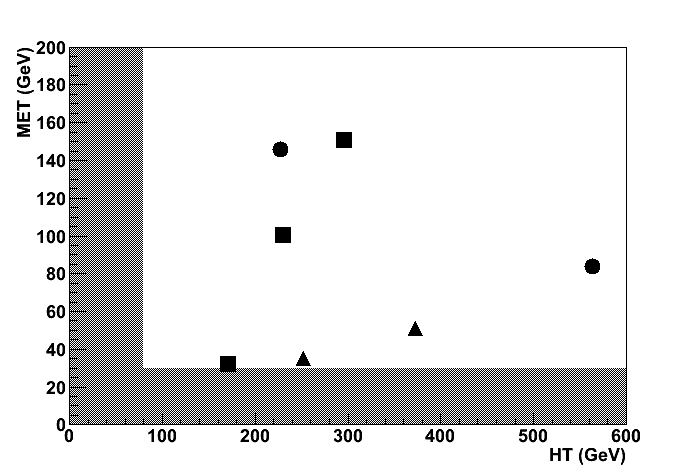
\includegraphics[width=0.48\linewidth]{figs/MetVsHt.png}
\caption{\label{fig:htvsmet}
Distribution of \met~~vs. $H_T$ for the 7 events in the baseline region
\met$> 30$ GeV and $H_T > 80$ GeV; $ee$ events: circles; $e\mu$ events: 
squares; $\mu\mu$ events: triangles.}
\end{center}
\end{figure}

\begin{figure}[h]
\begin{center}
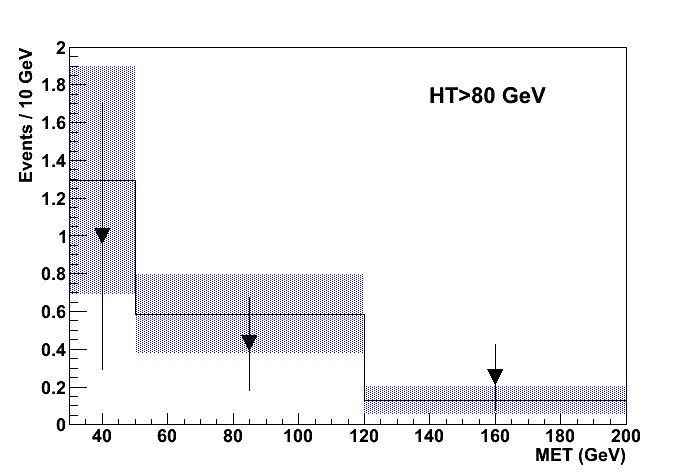
\includegraphics[width=0.48\linewidth]{figs/Met.png}
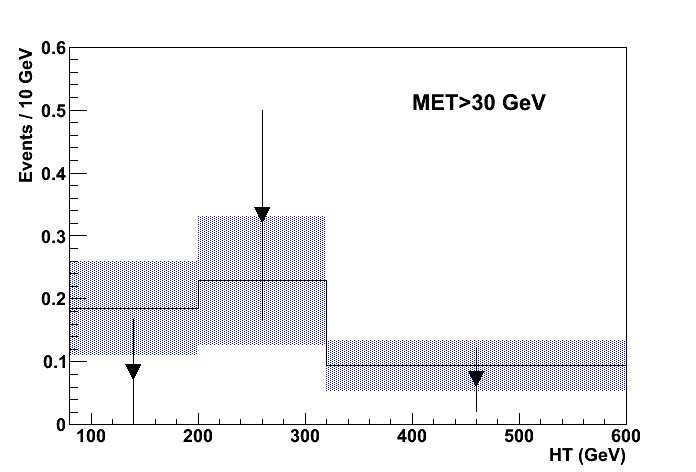
\includegraphics[width=0.48\linewidth]{figs/Ht.png}
\caption{\label{fig:htmet}
\met~~and $H_T$ distribution for the events in the baseline region (points).
Also shown as a histogram is the result of the background prediction.
The shading around the histogram represents the uncertainty
in the background prediction.}
\end{center}
\end{figure}


 




